\documentclass[conference]{IEEEtran}
\IEEEoverridecommandlockouts
% The preceding line is only needed to identify funding in the first footnote. If that is unneeded, please comment it out.
\usepackage{cite}
\usepackage{dblfloatfix}
\usepackage{amsmath,amssymb,amsfonts}
\usepackage{algorithmic}
\usepackage{listings}
\usepackage{graphicx}
\usepackage{textcomp}
\usepackage{xcolor}
\usepackage[utf8]{inputenc}

\usepackage{listings}
\usepackage{xcolor}

\definecolor{codegreen}{rgb}{0,0.6,0}
\definecolor{codegray}{rgb}{0.5,0.5,0.5}
\definecolor{codepurple}{rgb}{0.58,0,0.82}
\definecolor{backcolour}{rgb}{0.95,0.95,0.92}

\lstdefinestyle{mystyle}{
    backgroundcolor=\color{backcolour},   
    commentstyle=\color{codegreen},
    keywordstyle=\color{magenta},
    numberstyle=\tiny\color{codegray},
    stringstyle=\color{codepurple},
    basicstyle=\ttfamily\footnotesize,
    breakatwhitespace=false,         
    breaklines=true,                 
    captionpos=b,                    
    keepspaces=true,                 
    numbers=left,                    
    numbersep=5pt,                  
    showspaces=false,                
    showstringspaces=false,
    showtabs=false,                  
    tabsize=2
}

\lstset{style=mystyle}
\def\BibTeX{{\rm B\kern-.05em{\sc i\kern-.025em b}\kern-.08em
    T\kern-.1667em\lower.7ex\hbox{E}\kern-.125emX}}
\begin{document}

\title{Implementing K-Means Clustering\\
}

\author{\IEEEauthorblockN{Devopriya Tirtho}
\IEEEauthorblockN{16.02.04.033}
\IEEEauthorblockA{\textit{Department of Computer Science and Engineering} \\
\textit{Ahsanullah University of Science and Technology}\\
Dhaka, Bangladesh \\
}

}

\maketitle

\begin{abstract}
 \textbf{'Machine Learning'} is the kind of learning which tries to train a device according to learning to work smarter. In \textbf{Machine Learning}, there are two types of learning. One is \textbf{Supervised Learning} and the other one is \textbf{Unsupervised Learning}. In first intuition, we may think without any labelling how we can train the device to learn something. There are some advanced algorithms which are based on \textbf{Unsupervised Learning}. \textbf{K-Means Clustering} is one of them. In this experiment, we will implement the K-Means Clustering algorithm.
\end{abstract}

\begin{IEEEkeywords}
Machine Learning, K-Means Cluster, Unsupervised Learning, Supervised Learning.
\end{IEEEkeywords}

\section{Introduction}
\textbf{K-Means Clustering} is a form of \textbf{Unsupervised Learning}. We have already known about the \textbf{Supervised Learning}, now it is the time to work with \textbf{Unsupervised Learning}. In \textbf{Unsupervised Learning}, there is no labelled data. We have to predict the classes according to their happenings. In \textbf{K-Means Clustering}, we are given \textbf{K}  number of clusters to divide our datapoints. The clusters are generated according to their \textbf{mean} value, that is why this model is called \textbf{K-Means Clustering}. The distance measurement we consider here is the \textbf{Euclidean Distance} from one point to another. The word \textbf{cluster} means there are some datapoints together and the main goal is to keep the distance low of in-cluster points and keep the distance high of the clusters.

\section{Task}
As this classifier is a form of \textbf{unsupervised learning}, there is no labelled data. So, we are given some datapoints at random. These data have to be clustered. Here, there are some examples of our given datapoints:\\
$W$= $\{(-7.87157,-4.86573),(5.86288,0.99790),.....\}$\\
For implementing the \textbf{K-Means Clustering}, there are some gradually incremented tasks which we have to solve on the way of implementing. These tasks are:
\begin{itemize}  
\item Firstly, we have to take all the input datapoints from the file and plot the points.
\item Secondly, the implementation part comes. We have to implement the \textbf{K-Means Clustering} model with the cluster value of \textbf{k} which is taken from user.
\item Lastly, we have to color the corresponding datapoints according to clusters.

\end{itemize}
\section{Experimental Design}
\begin{itemize}  
\item For the first task, we have to plot the datapoints which are taken from the input file and visualize the occurances.
\begin{figure}[htb!]
\centerline{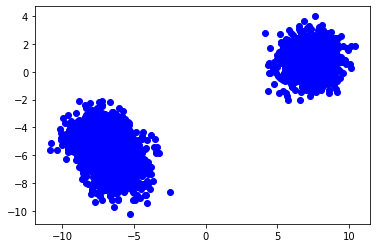
\includegraphics[scale=0.5]{51.png}}
\caption{Visualization of the Datapoints\\}
\label{fig}
\end{figure}

\item Now, it is the time for the implementation of  \textbf{K-Means Clustering} model. Before the implementation, we need to understand how the algorithm works.\\
\begin{figure}[htb!]
\centerline{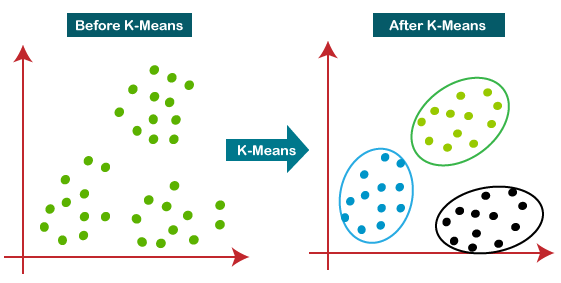
\includegraphics[scale=0.45]{52.png}}
\caption{K-Means Clustering\\}
\label{fig}
\end{figure}
   \begin{itemize}
     \item Firstly, we need to take the input of cluster number \textbf{K}
     \item Then, we have to find the centroids by shuffling the datapoints and take random datapoints as centroids.
	\item After that, we have to iterate over all the datapoints and keep changing the centroid according to the newest mean value. For finding the distance, we will follow the \textbf{Euclidean Distance's} value.
   \end{itemize}
\begin{equation}
\sqrt{\left(x_{2}-x_{1}\right)^{2}+\left(y_{2}-y_{1}\right)^{2}}
\end{equation}
	\item For stopping, we may define a fixed iteration number or we have to keep track of the changing datapoints and centroids. When there is no change in fixing the centroid, the algorithm stops.
Our main task is to plot the datapoints close to the centroids.



\item Finally, we need to color the corresponding datapoints of each cluster differently. \\
\begin{figure}[htb!]
\centerline{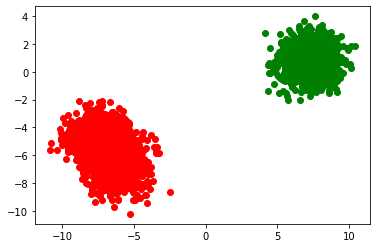
\includegraphics[scale=0.5]{53.png}}
\caption{Visualization of the Clusters\\}
\label{fig}
\end{figure}
\end{itemize}

\section{Result Analysis}
After implementing the algorithm, we have seen different colored datapoint at different clusters. From the picture, we can see that, datapoints which are very close to each other are colored in same and datapoints which are far, they are of different color. The in-cluster distance of the datapoints is less while, the distance between different clusters are high.
\section{Python Code}



\begin{lstlisting}
# -*- coding: utf-8 -*-
"""160204033_A2_05.ipynb

Automatically generated by Colaboratory.

Original file is located at
    https://colab.research.google.com/drive/1OKyARfCG4HyAg-Ff-MnHkmlsT_gSiIYP
"""

import io
import random 
import pandas as pd
import numpy as np
import matplotlib.pyplot as plt
data = pd.read_csv('data_k_mean.txt',sep=" ",header = None)
x=[i for i in data[0]]
y=[i for i in data[1]]
plt.plot(x ,y ,marker="o",linestyle = 'None',color="blue")

k = int(input("Enter the Value of Clusters: "))
datalen=len(data[0])
print(datalen)
centroids=[]
for i in range(k):
  index=random.randint(0,datalen-1)
  centroids.append([data[0][index],data[1][index]])
print(centroids)

import math
lst=[]
converge=False
for m in range (0,200):
  
  if(m>0):
    centroidsTmp=[]
    for j in range(k):
      classwisedata1=[i[0] for i in lst if i[2]==j]
      classwisedata2=[i[1] for i in lst if i[2]==j]
  
      centroidsTmp.append([sum(classwisedata1)/len(classwisedata1),sum(classwisedata2)/len(classwisedata2)])
    
    if(centroids==centroidsTmp):
      converge=True
    else:
      centroids=centroidsTmp
      
  if(converge):
    break
  lst=[]
  print("iteration: ",m)
  for i in range(0,datalen):
    distance=[]
    for j in range(k):
      distance.append(math.sqrt(pow(centroids[j][0]-data[0][i],2)+pow(centroids[j][1]-data[1][i],2)))
      

    lst.append([data[0][i],data[1][i],distance.index(min(distance))])  
  
  print(lst)

import matplotlib.pyplot as plt
st=['red','green','blue','yellow']
for i in range(k):
  x1=[j[0] for j in lst if j[2]==i ]
  y1=[j[1] for j in lst if j[2]==i ]
  colIndex=i%4
  plt.plot(x1,y1 ,marker="o",linestyle = 'None',color=st[colIndex])


\end{lstlisting}


\section{Conclusion}

\textbf{K-Means Classifier} is a classifier which is based on \textbf{Unsupervised Learning}. There are several classifiers, but \textbf{K-Means Classifier} works better and the algorithm is simple as well. The knowledge of implementation will help us to consturct other models in future.



\end{document}
